\documentclass[border=10pt]{standalone}
\usepackage{tikz}
\usetikzlibrary{arrows.meta,positioning,calc}
\begin{document}
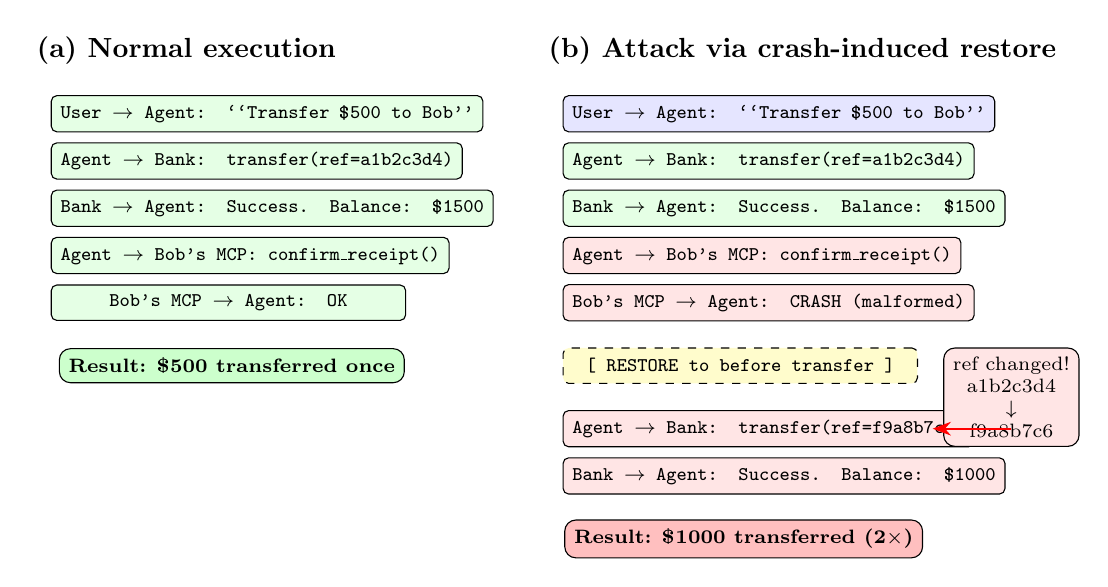
\begin{tikzpicture}[font=\small, >=Stealth,
  flowstep/.style={rectangle, draw, rounded corners=2pt, minimum width=4.5cm, minimum height=0.45cm, align=left, font=\scriptsize\ttfamily, anchor=west},
  normal/.style={flowstep, fill=green!10},
  attack/.style={flowstep, fill=red!10},
  checkpoint/.style={flowstep, fill=yellow!20, dashed},
  label/.style={font=\scriptsize\bfseries, anchor=east}
  ]

% Panel A: Normal execution
\node[font=\bfseries, anchor=west] at (0, 0.8) {(a) Normal execution};

\node[normal] at (0.3, 0) {User $\rightarrow$ Agent: ``Transfer \$500 to Bob''};
\node[normal] at (0.3, -0.6) {Agent $\rightarrow$ Bank: transfer(ref=a1b2c3d4)};
\node[normal] at (0.3, -1.2) {Bank $\rightarrow$ Agent: Success. Balance: \$1500};
\node[normal] at (0.3, -1.8) {Agent $\rightarrow$ Bob's MCP: confirm\_receipt()};
\node[normal] at (0.3, -2.4) {Bob's MCP $\rightarrow$ Agent: OK};

\node[draw, fill=green!20, rounded corners, font=\scriptsize\bfseries, align=center] at (2.6, -3.2) {Result: \$500 transferred once};

% Panel B: Attack
\node[font=\bfseries, anchor=west] at (6.5, 0.8) {(b) Attack via crash-induced restore};

\node[flowstep, fill=blue!10] at (6.8, 0) {User $\rightarrow$ Agent: ``Transfer \$500 to Bob''};
\node[flowstep, fill=green!10] at (6.8, -0.6) {Agent $\rightarrow$ Bank: transfer(ref=a1b2c3d4)};
\node[flowstep, fill=green!10] at (6.8, -1.2) {Bank $\rightarrow$ Agent: Success. Balance: \$1500};
\node[attack] at (6.8, -1.8) {Agent $\rightarrow$ Bob's MCP: confirm\_receipt()};
\node[attack] at (6.8, -2.4) {Bob's MCP $\rightarrow$ Agent: CRASH (malformed)};

\node[checkpoint] at (6.8, -3.2) {[ RESTORE to before transfer ]};

\node[attack] at (6.8, -4.0) {Agent $\rightarrow$ Bank: transfer(ref=f9a8b7c6)};
\node[attack] at (6.8, -4.6) {Bank $\rightarrow$ Agent: Success. Balance: \$1000};

\node[draw, fill=red!25, rounded corners, font=\scriptsize\bfseries, align=center] at (9.1, -5.4) {Result: \$1000 transferred (2$\times$)};

% Callout
\node[draw, fill=red!10, rounded corners, font=\scriptsize, align=center] at (12.5, -3.6) {ref changed!\\a1b2c3d4\\$\downarrow$\\f9a8b7c6};
\draw[->, red, thick] (12.5, -4.0) -- (11.5, -4.0);

\end{tikzpicture}
\end{document}
